\chapter{Monad Transformer}

Monad transformers offer an additional benefit to monadic programming: by providing a
library of different monads and types and functions for combining these monads, it is possible
to create custom monads simply by composing the necessary monad transformers. [Monad Transformers Step by Step]

\section{State Transformer}
A value of type \textbf{(ST a s)} is a computation which transforms a state index by type s ,and delivers a value of type a ,You can think of it as a box ,like this 

\begin{figure}[H]
  \centering
	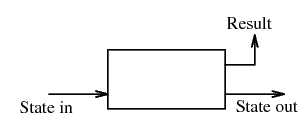
\includegraphics[width=0.60\textwidth]{pic/c3/state.png}
	\caption{Diagram illustrating a state monad}
\end{figure}
[lazy functional state thread]


\section{Error Transformer}


\section{Putting All Together}